% -------------------------------------------------------
% This plot is from DefElement (https://defelement.com)
% and is available under a Creative Commons Attribution
% 4.0 International (CC BY 4.0) license:
% https://creativecommons.org/licenses/by/4.0/
% -------------------------------------------------------
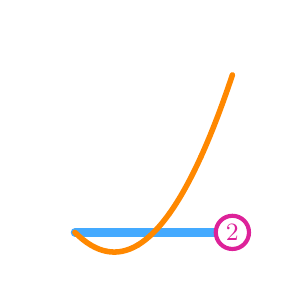
\begin{tikzpicture}[x=0.2mm,y=0.2mm]
\definecolor{color0}{HTML}{44AAFF}
\definecolor{color1}{HTML}{FF8800}
\definecolor{color2}{HTML}{DD2299}
\clip (0,0) rectangle (160,160.0);
\draw[color0,line width=3pt,line cap=round](30.0,30.0) -- (130.0,30.0);
\draw[color1,line cap=round,line width=2pt] (30.0,30.0) .. controls (36.666666666666664,23.333333333333332) and (43.333333333333336,19.333333333333336) .. (50.0,18.0);
\draw[color1,line cap=round,line width=2pt] (50.0,18.0) .. controls (56.66666666666667,16.666666666666664) and (63.33333333333333,18.0) .. (70.0,22.000000000000004);
\draw[color1,line cap=round,line width=2pt] (70.0,22.000000000000004) .. controls (76.66666666666666,26.000000000000004) and (83.33333333333334,32.66666666666667) .. (90.0,42.0);
\draw[color1,line cap=round,line width=2pt] (90.0,42.0) .. controls (96.66666666666666,51.33333333333333) and (103.33333333333333,63.33333333333333) .. (110.0,78.00000000000003);
\draw[color1,line cap=round,line width=2pt] (110.0,78.00000000000003) .. controls (116.66666666666667,92.66666666666669) and (123.33333333333333,110.0) .. (130.0,130.0);
\draw[color2,fill=white,line width=1.5pt] (130.0,30.0)circle (6pt);
\node[anchor=center] at (130.0,30.0) {\small\color{color2}2};
\end{tikzpicture}